\documentclass[journal,transmag]{IEEEtran}

% ..........................................................................
% Packages, configuration settings, and macro definitions.

\usepackage[pdftex]{graphicx}
\graphicspath{figures}
\DeclareGraphicsExtensions{.pdf,.jpeg,.png}

\usepackage[pdftex,rgb,dvipsnames,svgnames,hyperref,table]{xcolor}

\usepackage[pdftex,breaklinks=true,colorlinks=true,
	bookmarks=false,pdfhighlight=/O,
	urlcolor=DarkBlue,citecolor=DarkRed,linkcolor=DarkBlue]{hyperref}

\usepackage[cmex10]{amsmath}
\interdisplaylinepenalty=2500

\usepackage{amssymb}
\usepackage{amsfonts}
\usepackage{multicol}
\usepackage{multirow}
\usepackage{enumitem}
\usepackage{accsupp}
\usepackage{array}
\usepackage[caption=false,font=footnotesize]{subfig}
\usepackage{booktabs}
\usepackage{xspace}
\usepackage{soul}
\usepackage{url}
\usepackage{hyphenat}
\usepackage[english]{babel}

% Correct bad hyphenation here
\hyphenation{op-tical net-works semi-conduc-tor ana-ly-tics}

\usepackage{pdfcomment}
%\newcommand{\comment}[3]{\pdfmarkupcomment[markup=Highlight,color=yellow,author={#2}]{#1}{#3}}

\usepackage{tabularx}
% ..........................................................................
% Body.

\begin{document}

\markboth{IEEE Transactions on Biomedical Engineering}{2015 Whole-Cell Modeling Summer School meeting report}

\title{Combining standards for tomorrow's models: Report of the 2015 Whole-Cell Modeling Summer School}

\author{
	\IEEEauthorblockN{
		Dagmar Waltemath\IEEEauthorrefmark{1},
		Falk Schreiber\IEEEauthorrefmark{2,3}, 
		Jonathan R. Karr\IEEEauthorrefmark{4}, 
%		Michael Hucka\IEEEauthorrefmark{5},
%        Chris J. Myers\IEEEauthorrefmark{6},
%        Frank T. Bergmann\IEEEauthorrefmark{5,7,8},\\
%        Vijayalakshmi Chelliah\IEEEauthorrefmark{9},
%        Marcus Krantz\IEEEauthorrefmark{10},
%        Wolfram Liebermeister\IEEEauthorrefmark{11},
%        Pedro Mendes\IEEEauthorrefmark{12--15},
                %        Pinar Pir\IEEEauthorrefmark{16},
                Rafael S. Costa\IEEEauthorrefmark{19},
                Sucheendra K. Palaniappan\IEEEauthorrefmark{17}, \\
                Kieran Smallbone\IEEEauthorrefmark{18}, 
         Markus Wolfien\IEEEauthorrefmark{1}, and 
         2015 Whole-Cell Modeling Summer School Consortium\IEEEauthorrefmark{5} 
        }
	
	\IEEEauthorblockA{\IEEEauthorrefmark{1}Department of Systems Biology and Bioinformatics, University of Rostock}
	\IEEEauthorblockA{\IEEEauthorrefmark{2}Clayton School of Information Technology, Monash University}
    \IEEEauthorblockA{\IEEEauthorrefmark{3}Institute of Computer Science, Martin Luther University Halle-Wittenberg}    
	\IEEEauthorblockA{\IEEEauthorrefmark{4}Department of Genetics \& Genomic Sciences, Icahn School of Medicine at Mount Sinai} 
        %New York, NY 10029 USA\\Email: \href{mailto:karr@mssm.edu}{karr@mssm.edu}
%    \IEEEauthorblockA{\IEEEauthorrefmark{5}Department of Computing and Mathematical Sciences, California Institute of Technology} 
        %1200 East California Boulevard, Pasadena, CA 91125, USA
%    \IEEEauthorblockA{\IEEEauthorrefmark{6}Department of Electrical and Computer Engineering, University of Utah} 
        %Salt Lake City, Utah 84112, USA
%    \IEEEauthorblockA{\IEEEauthorrefmark{7}BioQuant, University of Heidelberg} 
        %Heidelberg , Germany
%    \IEEEauthorblockA{\IEEEauthorrefmark{8}Centre for Organismal Studies, University of Heidelberg} 
%    \IEEEauthorblockA{\IEEEauthorrefmark{9}European Molecular Biology Laboratory, European Bioinformatics Institute} 
        %Wellcome Trust Genome Campus, Hinxton, Cambridge CB10 1SD, UK viji@ebi.ac.uk.
%    \IEEEauthorblockA{\IEEEauthorrefmark{10}Department of Biology, Humboldt University of Berlin} 
        %Berlin, Germany
%    \IEEEauthorblockA{\IEEEauthorrefmark{11}Institute of Biochemistry, Charit\'e Medical University of Berlin} 
        %10117 Berlin, Germany
%    \IEEEauthorblockA{\IEEEauthorrefmark{12}Manchester Institute of Biotechnology, University of Manchester} 
%    \IEEEauthorblockA{\IEEEauthorrefmark{13}School of Computer Science, University of Manchester}     
%    \IEEEauthorblockA{\IEEEauthorrefmark{14}Center for Quantitative Medicine, University of Connecticut Health Center}
%    \IEEEauthorblockA{\IEEEauthorrefmark{15}Department of Cell Biology, University of Connecticut Health Center}
        %131 Princess Street, Manchester, M1 7DN, UK. pedro.mendes@manchester.ac.uk
        %Farmington, Connecticut, USA
%    \IEEEauthorblockA{\IEEEauthorrefmark{16}Babraham Institute}
    \IEEEauthorblockA{\IEEEauthorrefmark{17} INRIA, Campus de Beaulieu, Rennes, France}
    %
    \IEEEauthorblockA{\IEEEauthorrefmark{18}  Manchester Centre for Integrative Systems Biology, University of Manchester, U.K.}
    %
    \IEEEauthorblockA{\IEEEauthorrefmark{19}  IDMEC / IST - University of Lisbon, Portugal}
    %
    \IEEEauthorblockA{\IEEEauthorrefmark{5}Membership of the 2015 Whole-Cell Modeling Summer School Consortium is listed in Table~SI}
    %
	\thanks{Corresponding author email: \href{mailto:dagmar.waltemath@uni-rostock.de}{dagmar.waltemath@uni-rostock.de}}
}

\IEEEtitleabstractindextext{
	\begin{abstract}
	Computational modeling is an increasingly important tool for biological research, bioengineering, and medicine. 
	Recently, researchers developed the first whole-cell model which represents every individual molecular species and gene function.
	However, significant work remains to develop fully complete and accurate models. 
	We organized the 2015 Whole-Cell Modeling Summer School to teach students the latest cell modeling methods, as well as to assess the need for whole-cell modeling standards.
	We found that standards would accelerate whole-cell modeling and that our current standards SBML, SED-ML, and SBGN must be expanded to support whole-cell modeling.
	% One major criticism of these standards is that they lag behind current developments and thereby may not be suitable to fully encode today's models. 
    % To overcome this problem, the applicants, under the guidance of the COMBINE effort, will organize a summer school for standard developers and modelers, i.e., users of these standards. 
    % The main goal is to explore the expressivity of current standard formats using the example of the famous whole-cell model, which has not yet been encoded in a standard format.
	\end{abstract}
	
	% Note that keywords are not normally used for peer review papers.
	\begin{IEEEkeywords}
	Whole-cell modeling, Systems biology, Computational biology, Mathematical modeling, Simulation, Standards, Education
	\end{IEEEkeywords}
}

\maketitle
\IEEEdisplaynontitleabstractindextext
\IEEEpeerreviewmaketitle

\section{Introduction}

% The very first letter is a 2 line initial drop letter followed by the rest of the first word in caps.
% 
% form to use if the first word consists of a single letter:
% \IEEEPARstart{A}{demo} file is ....
% 
% form to use if you need the single drop letter followed by normal text (unknown if ever used by IEEE):
% \IEEEPARstart{A}{}demo file is ....
% 
% Some journals put the first two words in caps:
% \IEEEPARstart{T}{his demo} file is ....
% 
% Here we have the typical use of a "T" for an initial drop letter and "HIS" in caps to complete the first word.
% is a report of the VW Whole-cell Summer School held in Rostock during April 2015.

\IEEEPARstart{O}{ver} the past twenty years, computational modeling has become an essential and powerful tool for biological research, bioengineering, and medicine to analyze high-throughput molecular measurements and understand the molecular details of complex biological systems. 
Computational modeling has already been used to identify new metabolic genes~\cite{Reed2006}, add metabolic pathways to bacteria~\cite{Lee2009}, and identify potential new antimicrobial drug targets~\cite{Lee2012}. 
Computational models also have the potential to enable bioengineers to design new microorganisms for industrial applications such as chemical synthesis, biofuel production, and waste decontamination, as well as to enable clinicians to design personalized medical therapies tailored to each individual patient's unique genome. 
Realizing this potential requires more comprehensive and accurate computational models which are capable of predicting cellular behavior from genotype, as well as standardized methods for exchanging models, simulation experiments, and model visualizations~\cite{Macklin2014,Karr2015,hucka2015promoting,Klipp07}.

Recently, researchers at Stanford University developed the first whole-cell model of the gram-positive bacterium \textit{Mycoplasma genitalium}~\cite{Karr2012}. 
The model represents the life cycle of a single Mycoplasma cell including the copy number dynamics of each metabolite, RNA, and protein species and accounts for every known gene function. 
The model is comprised of 28 sub-models, each of which was implemented using different mathematical representations including ordinary differential equations (ODEs), flux balance analysis (FBA), and Boolean rules (BRs), and trained using different experimental data. 

The \textit{M. genitalium} whole-cell model was implemented in MATLAB, is available open-source under the MIT license, and is extensively documented. 
This has enabled other researchers to use the model for their own research and enabled educators to use the model to teach systems biology. 

Although MATLAB is commonly used by academic researchers, it is proprietary and expensive. In addition, because many of the biological details of the model are intertwined with the MATLAB code, significant domain expertise is currently required to understand, use, or modify the Mycoplasma model or construct new whole-cell models. 
Transparent whole-cell modeling standards and simulation tools are needed to enable more researchers to develop and use whole-cell models for their own research. 
Such standards would accelerate the whole-cell modeling field. They would enable researchers to develop models more quickly, more deeply explore model predictions, and more rigorously evaluate models. Furthermore, they would enable researchers to contribute whole-cell models to model repositories such as BioModels~\cite{li2010biomodels} which in turn, would make models more searchable, retrievable, and comparable.

Several systems biology standards have already been developed by the COmputational Modeling in BIology NEtwork (COMBINE)~\cite{le2011meeting} including the Systems Biology Markup Language (SBML)~\cite{hucka2003}, the Cell Markup Language (CellML)~\cite{hedley_2001b}, the Simulation Experiment Description Markup Language (SED-ML)~\cite{sedml2011}, and the Systems Biology Graphical Notation (SBGN)~\cite{LeNovereHMMSS09}. SBML and CellML are standard languages for describing mathematical models including ODE, logical, and FBA models. Both have been used to build hundreds of models of various intracellular pathways. 
However, neither language supports several of the features needed for whole-cell modeling including large, sparsely occupied state spaces and multi-algorithm simulations. 
SED-ML is a standard language for describing computational experiments. SED-ML enables computational scientists to reproduce simulations by describing simulation setups in detail, including the simulation algorithm and every parameter value. 
SBGN is a standard language for describing visual representations of models. SBGN also has some restrictions regarding the visualization of whole-cell models, in particular there is no support for mixed diagrams or for generic reactions.
Taken together, further work is needed to expand the capabilities of the current systems biology standard languages to support whole-cell modeling.

We organized the 2015 Whole-cell Modeling Summer School to train students in whole-cell modeling and assess the limitations of the current systems biology standards for whole-cell modeling. 
The first and foremost goal of the school was to train young researchers how to build whole-cell models, including how to develop sub-models of individual cellular pathways using different mathematical formalisms; how to assemble sub-models into a single model; and how to encode models using SBML, simulate models using SED-ML, visualize models using SBGN, and link model entities to semantic annotations in controlled systems biology vocabularies \cite{courtot2011a}. 
The second goal of the school was to identify how the SBML, SED-ML, and SBGN languages must be expanded to support whole-cell and other state-of-the-art modeling.
The third goal of the school was to reimplement the \textit{M. genitalium} whole-cell model using SBML.

The summer school arose from discussions at the 2012 COMBINE tutorial~\cite{COMBINE2012} about how to best engage and inform modelers about COMBINE standards. The discussions concluded that a summer school focused on a specific well-known model would be an excellent forum to educate young researchers on how to build models and encode them using COMBINE standards. Dagmar Waltemath and Falk Schreiber organized the school over the following three years, obtained funding for the school from the Volkswagen Foundation, recruited nine tutors with broad experience in computational systems biology and COMBINE standards to help teach the school, and selected 45 students to attend the school.

Here, we report the educational and scientific outcomes of the summer school. 
First, we summarize the format and content of the summer school. 
Second, we describe the educational outcomes of the school and our progress toward encoding the \textit{M. genitalium} whole-cell model using SBML. 
Third, we describe the limitations we learned for using SBML to encode whole-cell models. We also describe several lessons that we learned about how to successfully organize a summer school. 
Lastly, we outline a path toward expanding the SBML, SED-ML, and SBGN standards to support whole-cell modeling and encoding the \textit{M. genitalium} whole-cell model using SBML.

\section{The 2015 Whole-Cell Modeling Summer School}
The goal of the summer school was to teach students how to build models and encode models using COMBINE standards through encoding the \textit{M. genitalium} model using only standard representation formats and open-source simulation software. 
To achieve this goal, we devoted most of the five-day school to hands-on active learning sessions in which ten groups of 4-5 students, each led by one tutor, were tasked with encoding parts of the \textit{M. genitalium} model using COMBINE standards. 
Prior to the school, we assigned students, tutors, and sub-models to groups based on a survey of the students' backgrounds and interests. 
The groups also began meeting online using Google Hangouts and encoding sub-models prior to the school. 
Jonathan Karr also worked with all of the groups to teach students about cell modeling. 
Table~SI lists the ten groups and all of the students and tutors. 
In addition to the hands-on active learning sessions, the school featured two lectures on whole-cell modeling and modeling standards from Jonathan Karr and Michael Hucka, two group discussions on model integration, daily oral progress reports from each of the working groups, a poster session, and three networking activities.

\subsection{Introductory lectures}
We began the school with two lectures to introduce the students to whole-cell modeling and the existing systems biology standards. Jonathan Karr from the Icahn School of Medicine at Mount Sinai, USA presented an overview of whole-cell modeling, the latest methods for constructing whole-cell models, the \textit{M. genitalium} whole-cell model and his own research on developing whole-cell models for bioengineering and precision medicine. Michael Hucka from the California Institute of Technology, USA presented an overview of the main systems biology standards SBML, SED-ML, and SBGN; the most popular open-source software tools which support these standards; and the COMBINE initiative.

\subsection{Group discussions}
In addition to the introductory lectures, we organized three group discussions on three common SBML encoding problems. The first discussion focused on how to sample from random distributions within the context of SBML. The second discussion focused on the interfaces that sub-models must expose to facilitate integration into a single model. The third discussion focused on how to model large, sparsely occupied state spaces such as that which represents the locations of DNA-bound proteins.

\subsection{Active learning sessions}
The majority of days 2-4 of the school were dedicated to hands-on active learning sessions in which students learned about whole-cell modeling and the COMBINE standards by encoding parts of the \textit{M. genitalium} whole-cell model using SBML. Specifically, eight of the ten groups were responsible for encoding one or more sub-models. The ninth group focused on developing a standards-compliant scheme for integrating SBML-encoded sub-models into a single model. This group was responsible for defining the sub-model interfaces. The tenth group focused on helping the other groups document and visualize their sub-models using SBGN. Each group was led by an experienced tutor.

The groups pursued various strategies to encode the sub-models using COMBINE-compliant representations. Several of the groups encoded sub-models by first reading the sub-model documentation, second drawing pathway maps using software tools such as Cell Designer~\cite{funahashi2008celldesigner} and VANTED~\cite{Rohn2012}, and then writing scripts to automatically generate SBML representations from their maps. Other groups used modeling software tools such as COPASI~\cite{Mendes2009} and BioUML~\cite{Kolpakov2006} to encode sub-models based on their documentation. A third set of groups encoded sub-models by converting the original MATLAB code to SBML. These groups then automatically generated SBGN maps from their SBML to better understand their sub-models.

\subsection{Progress reports}
We concluded each day with brief oral progress presentations from one member of each of the ten groups. These progress reports facilitated discussion on common standards encoding challenges, provided groups opportunities to get feedback from the rest of the school, and helped the integration group plan the assembly of the integrated model. On the first day, the groups presented overviews of the biology of their sub-models and their progress to date. On the last day, the groups summarized their progress from the school and their plan to complete their sub-model encoding. Throughout the school, each student presented at least once.

\subsection{Poster session}
To provide students opportunities to share their own research, we organized a poster session on the second night of the school. 
27 students presented posters. Many of the students presented projects on whole-cell modeling or other computational systems biology projects.

\subsection{Networking activities}
We organized several social activities to facilitate student networking. On the first night, we organized a dinner reception. On the third night, we organized a city tour led by a local guide. On the last evening, we organized a group dinner and dance party.

\section{Results}

\subsection{Educating young systems biologists}
The primary goal of the summer school was to educate young scientists on how to build and apply whole-cell models. Because the students came from a variety of backgrounds ranging from computer science to biology, the tutors provided students one-on-one instruction on molecular cell biology; common dynamical modeling methods including ODEs, FBA, and BRs; model integration; and the SBML, SED-ML, and SBGN systems biology standards.

%\comment{
Following the summer school, most of the students reported that they gained deeper knowledge of whole-cell modeling. 
They also reported increased appreciation for the importance of reproducibility and increased understanding of the SBML, SED-ML, and SBGN standards and how they facilitate reproducible computational science.
In addition, many students reported that they learned a lot about open-source modeling software tools which are applicable to their graduate research.

The students also reported that the course was a valuable networking event. 
Students reported that they had many opportunities to connect with other young computational systems biology researchers from around the world.
In particular, students found that the poster session provided them an opportunity to share their own work and get valuable feedback from each other, the tutors, and other scientists from the University of Rostock.
Several of the students also reported that the course introduced them to other opportunities to learn more about whole-cell modeling including open postdoctoral positions and the 2016 Whole-Cell Modeling Summer School which Jonathan Karr, Luis Serrano, Maria Lluch-Senar, and Javier Carrera are organizing in Barcelona, Spain.

% \subsection{\comment{Setting the goal}{Karr}{I would probably eliminate this section and merge the thoughts about code committed to GitHub with the following section. 
% If the goal was to create a working model, then the goal wasn't met and likely will never be met. Probably very few of the SBML sub-models actually work. 
% None of them have been tested to any degree. And a lot of work remains to integrate them. 
% I definitely wouldn't claim the sub-models will be published by the fall because this is not likely to happen.}}
% \comment{Setting the goal}{Waltemath}{Agreed}

% The goal to encode the whole-cell model was ambitious from the beginning, but the expectations have been more than met. 
% All participants dedicated their full time to working on the project, preparing initial results weeks beforehand, and even worked long hours. 
% The achieved results are of high quality and the spirit at the summer school was very positive over the whole week. 
% With 3 more days on the same project, we would have been able to test and then publish the 28 modules. 
% The final state after one week is that all material is there, but the modules need to be tested and integrated. 
% Several weeks after the summer school, the activity on the Git project is still high, and it can be expected that we will finish these two tasks before summer. 
% The modules shall be published in BioModels Database by autumn 2015. 

\subsection{Progress toward an SBML-encoded whole-cell model}
In addition to training young systems biology researchers, the course produced preliminary SBML and SBGN-ML versions of each of the \textit{M. genitalium} whole-cell model sub-models.
Since the course, the project groups have continued to meet online to complete the encoding and testing of their sub-models.
We plan to complete the encoding and integration of the advanced sub-models into a single model in a two-days satellite meeting to the COMBINE in October 2015. 
%into a single model within the next few months.

The sub-models and integrated model will be COMBINE-compliant, and simulatable with open-source software tools such as COPASI, BioUML, and iBioSim~\cite{Stevens2013}.
The sub-models and integrated model will be available open-source at \url{http://github.com/whole-cell-tutors/wholecell} and the BioModels database.
We believe the sub-models and integrated model will be a valuable community resource which will enable other scientists to develop, expand, and apply whole-cell models to their own research.

\section{Lessons learned}

\subsection{Limitations of SBML, SED-ML, and SBGN for whole-cell modeling}
Prior to the summer school, SBML, SED-ML, and SBGN had never been used to represent similarly large or complex models. 
Consequently, the summer school revealed several limitations of SBML, SBGN, and the existing COMBINE-compliant software for large models.
First, no COMBINE-compliant software supports multi-algorithm models such as the \textit{M. genitalium} whole-cell model. 
Second, SBML does not support sparse representations of large, combinatorial state spaces. Consequently, every state space must be enumerated. For the case of the \textit{M. genitalium} model, this means that the chromosome state space must be enumerated, resulting in millions of state variables and unmanageably large XML files.
Third, the core SBML language does not support arrays. Consequently, matrix operations that were efficiently implemented and executed in MATLAB, must be enumerated, resulting in verbose, opaque SBML files and inefficient simulations.
Fourth, SBML does not support random number generation which is required to encode many of the sub-models. Consequently, many of the sub-models must be recast as Gillespie algorithm simulations to be supported by SBML.

The summer school also revealed  limitations of SBGN for whole-cell models. 
First, whole-cell modeling requires SBGN maps which contain a mixture of Process Description, Entity Relationship, and Activity Flow nodes. Currently, SBGN maps can only contain one of these three types of nodes.
Second, whole-cell modeling demands improved support for automatic layout of large maps. The layout algorithms available are mostly not tailored to the specific networks occurring within a whole-cell model. 
Third, to reduce the complexity it would be helpful to provide generic forms of other entities in the same map, an issue already discussed within the SBGN community.

Most importantly, the summer school facilitated discussions among modelers, software tools developers, and model curators about how to best overcome these limitations.

\subsection{Organizing a summer school}
We also learned several valuable lessons about how to organize a productive, educational summer school.
First, we found that summer schools must have clear learning objectives.
Second, we found that students greatly enjoy hands-on active learning. 
Furthermore, we found that a high teacher to student ratio and a flexible schedule are necessary to successfully run open-ended project-based courses.
Third, we found that students should be divided into multidisciplinary teams. 
This enables students to learn from other scientists with alternative perspectives from other fields and builds strong teams that are well-equipped to solve difficult problems.
In the case of this summer school, it also enabled us to quickly assess potential expansions to the SBML language to support whole-cell models from multiple perspectives, ensuring that the expanded standards will meet the needs of modelers, software developers, and model curators.
Fourth, we found that social activities greatly enhance summer schools by encouraging informal networking interactions among students.
Lastly, we found that summer schools must have generous financial support. This enables organizers to accept students irrespective of their funding status. In turn, this enables the course to include a broader range of students than would otherwise be possible.

\section{Future steps}

The summer school made significant strides toward expanding the whole-cell modeling field by educating 45 young scientists in multi-algorithm modeling. 
The students had two introductory lectures which outlined the whole-cell modeling field and the existing systems biology standards; three discussions on model integration and how to efficiently represent large state spaces; and three full days of hands-on active learning exercises to recode sub-models using SBML. 
We are organizing a second meeting in conjunction with the 2015 COMBINE conference in Salt Lake City, USA to finish recoding and testing the sub-models.
In addition, Jonathan Karr, Luis Serrano, Maria Lluch-Senar, and Javier Carrera are organizing a second whole-cell modeling summer course in Barcelona in April 2016 which will focus on the theory of whole-cell modeling. 
Chris Myers at the University of Utah, USA and Vincent Danos at the National Centre for Scientific Research, France have also begun to offer graduate courses in whole-cell modeling.

Additional summer schools and courses are needed to provide students deeper theoretical training in the mathematical foundation of whole-cell modeling, as well as practical training in the construction of large dynamical models. These courses should provide students opportunities to learn about techniques for integrating multiple sub-models and resolving conflicts including state locking, adaptive time-stepping, controllers and semaphores; how to identify the parameters of large models including numerical optimization, distributed optimization, and model reduction; and how to test models using unit testing and continuous integration. 

The summer school made also significant strides toward reimplementing the \textit{M. genitalium} whole-cell model using SBML and COMBINE-compliant software. However, significant work remains to expand the SBML language to support whole-cell models, recode the \textit{M. genitalium} model using SMBL, and develop COMBINE-compliant software programs which are capable of efficiently simulating multi-algorithm models. Currently, we are working to finish recoding the sub-models using SBML and mapping each of the sub-models using SBGN. Since the Rostock meeting, the working groups have continued to meet virtually through Google Hangouts and share materials using GitHub and Google Drive. Several of the students and tutors also plan to participate in a second working meeting in conjunction with the COMBINE conference in Salt Lake City, USA in October 2015. We plan to publish these sub-models through the BioModels database along with tests implemented using SED-ML. 

Ultimately, we hope to integrate the individual sub-models into a single SBML-encoded model using the SBML-comp package. To achieve this, we must expand the SBML language to support multi-algorithm models and efficiently represent large, combinatorial state spaces. We plan to present proposals to expand SBML to support these features at the 2015 COMBINE conference in Salt Lake City, USA.

\section{Conclusion}
We believe that whole-cell modeling has the potential to be an important tool for biological discovery, bioengineering, and medicine.
Achieving this potential requires improved standards for transparently communicating whole-cell models, as well as COMBINE-compliant software for reproducibly simulating whole-cell models.
In turn, this requires expanding the whole-cell modeling field including training young researchers in whole-cell modeling.

We organized the 2015 Whole-Cell Modeling Summer School to train young researchers how to build whole-cell models using standardized languages through hands-on experience recoding the \textit{M. genitalium} whole-cell model using SBML. 
The school brought together 45 students including modelers, modeling software developers, and model curators. 
The school successfully trained 45 students, made significant progress toward recoding the \textit{M. genitalium} whole-cell model using SBML, and initiated a conversation about how to expand the SBML language to support multi-algorithm whole-cell models. 
We plan to publish the recoded sub-models through the BioModels database in the Fall and hope to eventually combine the SBML-encoded sub-models into a single model. 
We also plan to propose extensions to the SBML language to support whole-cell models at the 2015 COMBINE meeting in Salt Lake City, USA and to disseminate the proposed extensions through EraNet SysBio~\cite{ERASysBio2015}, CaSYM~\cite{CaSYM2015} and ISBE~\cite{Wolkenhauer2009}.
Finally, we hope the summer school will be the first of many whole-cell modeling meetings and courses.

\section*{Acknowledgments}
The course was supported by a grant from the Volkswagen Foundation to DW and FS. JRK was supported by a James S. McDonnell Foundation Postdoctoral Fellowship Award in Studying Complex Systems.

\ifCLASSOPTIONcaptionsoff
  \newpage
\fi

\bibliographystyle{IEEEtran}
\bibliography{IEEEabrv,report}

% biography section
% 
% If you have an EPS/PDF photo (graphicx package needed) extra braces are needed around the contents of the optional argument to biography to prevent
% the LaTeX parser from getting confused when it sees the complicated \includegraphics command within an optional argument. (You could create
% your own custom macro containing the \includegraphics command to make things simpler here.)

\begin{IEEEbiography}[{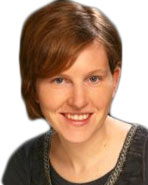
\includegraphics[width=1in,height=1.25in,clip,keepaspectratio]{photos/waltemath.jpg}}]{Dagmar Waltemath}
received her Ph.D. in Computer Science from the University of Rostock, Germany in 2011. 
Dr.~Waltemath is a Junior Research Group Leader in the Department of Systems Biology and Bioinformatics at the University of Rostock. 
Her group focuses on developing methods to reproducibly simulate computational biology models including managing, annotating, searching and retrieving models.
Dr.~Waltemath is also a COMBINE Coordinator and an SBML Editor. 
Contact: \href{mailto:dagmar.waltemath@uni-rostock.de}{dagmar.waltemath@uni-rostock.de}.
\end{IEEEbiography}

\begin{IEEEbiography}[{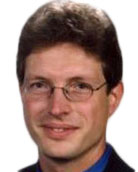
\includegraphics[width=1in,height=1.25in,clip,keepaspectratio]{photos/schreiber.jpg}}]{Falk Schreiber} 
received his Ph.D. (2001) and habilitation (2006) in Computer Science from the University of Passau, Germany. 
He is a Professor in the Faculty of Information Technology at Monash University, Australia, and an Adjunct Professor in the Institute of Computer Science at Martin Luther University Halle-Wittenberg, Germany. 
His research is focused on visual computing and visual analysis of biological data, analysis of the structure and dynamics of biological networks, integration of multimodal data,  standards for systems biology and modeling of metabolism. 
He is a COMBINE Coordinator and has been a SBGN Editor.
Contact: \href{mailto:falk.schreiber@monash.edu}{falk.schreiber@monash.edu}.
\end{IEEEbiography}

\begin{IEEEbiography}[{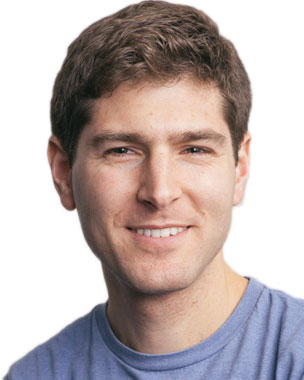
\includegraphics[width=1in,height=1.25in,clip,keepaspectratio]{photos/karr.jpg}}]{Jonathan R. Karr}
received his Ph.D. in Biophysics and M.S. in Medicine from Stanford University, USA in 2014 and his B.S.s in Physics and Brain \& Cognitive Sciences from the Massachusetts Institute of Technology, USA in 2006. 
Dr. Karr is a Fellow at the Icahn School of Medicine at Mount Sinai, USA. 
His research focuses on the development of comprehensive whole-cell computational models and their applications to bioengineering and medicine. 
Contact: \href{mailto:karr@mssm.edu}{karr@mssm.edu}.
\end{IEEEbiography}

\begin{IEEEbiography}[{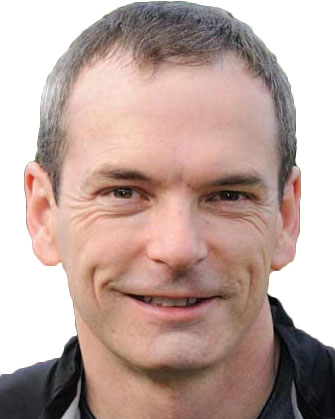
\includegraphics[width=1in,height=1.25in,clip,keepaspectratio]{photos/hucka.jpg}}]{Michael Hucka}
received his Ph.D. in Electrical Engineering and Computer Science from the University of Michigan in 1998 and his B.S.s in Computer Science and Electrical Engineering in 1986.
Dr. Hucka is a Member of the Professional Staff of the California Institute of Technology.
Contact: \href{mailto:mhucka@caltech.edu}{mhucka@caltech.edu}.
\end{IEEEbiography}

\begin{IEEEbiography}[{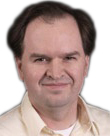
\includegraphics[width=1in,height=1.25in,clip,keepaspectratio]{photos/myers.jpg}}]{Chris J. Myers}
received his Ph.D. in Electrical Engineering from Stanford University in 1995 and his B.S.s in Electrical Engineering and Chinese History from the California Institute of Technology in 1991.
Dr. Myers is a Professor of Electrical and Computer Engineering at the University of Utah.
Contact: \href{mailto:myers@ece.utah.edu}{myers@ece.utah.edu}.
\end{IEEEbiography}

\begin{IEEEbiography}[{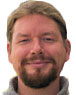
\includegraphics[width=1in,height=1.25in,clip,keepaspectratio]{photos/bergmann.jpg}}]{Frank T. Bergmann}
received his Ph.D. in Computational and Systems Biology from Claremont Graduate University in 2010 and his M.S. in Computer Science from Goethe University Frankfurt in 2004.
Dr. Bergmann is a Software Developer at the California Institute of Technology and a Member of the Scientific Staff at the University of Heidelberg.
Contact: \href{mailto:fbergman@caltech.edu}{fbergman@caltech.edu}.
\end{IEEEbiography}

\begin{IEEEbiography}[{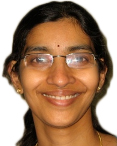
\includegraphics[width=1in,height=1.25in,clip,keepaspectratio]{photos/chelliah.jpg}}]{Vijayalakshmi Chelliah}
received her Ph.D. in Structural Bioinformatics \& Computational Biology from the University of Cambridge in 2005 and her B.Sc. in Mathematics, Physics and Computer Science from Manonmaniam Sundaranar University in 1995.
Dr. Chelliah is a Senior Scientific Curator at the European Bioinformatics Institute.
Contact: \href{mailto:viji@ebi.ac.uk}{viji@ebi.ac.uk}.
\end{IEEEbiography}

\begin{IEEEbiography}[{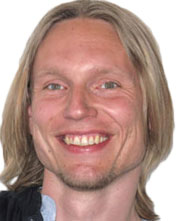
\includegraphics[width=1in,height=1.25in,clip,keepaspectratio]{photos/krantz.jpg}}]{Marcus Krantz}
received his Ph.D. in Microbiology from the University of Gothenburg in 2005.
Dr. Krantz is a Junior Research Group Leader at the Humboldt University of Berlin.
Contact: \href{mailto:marcus.krantz@biologie.hu-berlin.de}{marcus.krantz@biologie.hu-berlin.de}.
\end{IEEEbiography}

\begin{IEEEbiography}[{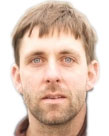
\includegraphics[width=1in,height=1.25in,clip,keepaspectratio]{photos/liebermeister.jpg}}]{Wolfram Liebermeister}
received his Ph.D. in Theoretical Biophysics from the Humboldt University of Berlin and his B.S. in Physics from the University of T\"ubingen.
Dr. Liebermeister is a Postdoctoral Fellow at the Charit\'e Medical University of Berlin.
Contact: \href{mailto:wolfram.liebermeister@charite.de}{wolfram.liebermeister@charite.de}.
\end{IEEEbiography}

\begin{IEEEbiography}[{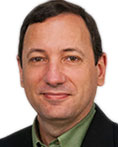
\includegraphics[width=1in,height=1.25in,clip,keepaspectratio]{photos/mendes.jpg}}]{Pedro Mendes}
received his Ph.D. in Biological Sciences from the University of Wales Aberystwyth in 1994 and his B.Sc in Biochemistry from the University of Lisbon in 1988.
Dr. Mendes is a Professor of Computer Science at the University of Manchester and a Professor of Cell Biology at the University of Connecticut Health Center.
Contact: \href{mailto:pedro.mendes@manchester.ac.uk}{pedro.mendes@manchester.ac.uk}.
\end{IEEEbiography}

\begin{IEEEbiography}[{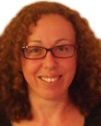
\includegraphics[width=1in,height=1.25in,clip,keepaspectratio]{photos/pir.jpg}}]{Pinar Pir}
received her Ph.D. in Chemical Engineering from Bo\v{g}azi\c{c}i University in 2005. 
Dr. Pir is Postdoctoral Research Associate at the Babraham Institute.
Contact: \href{mailto:pp305@cam.ac.uk}{pp305@cam.ac.uk}.
\end{IEEEbiography}

\begin{IEEEbiography}[{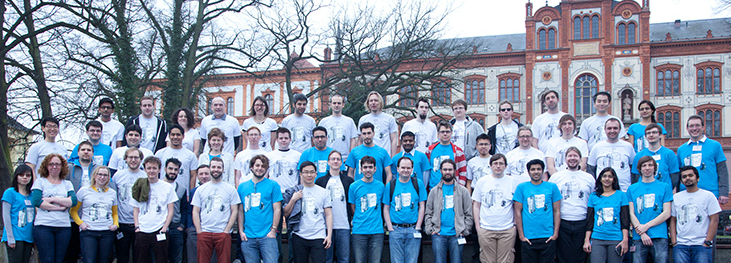
\includegraphics[width=3.48in,keepaspectratio]{photos/group.jpg}}]{}
~\\
~\\
~\\
~\\
~\\
~\\
~\\
~\\
~\\
~\\
~\\
\textbf{2015 Whole-Cell Modeling Summer School Consortium} includes the 56 researchers listed in Table~SI who organized and attended the 2015 summer school.
\end{IEEEbiography}


% You can push biographies down or up by placing a \vfill before or after them. The appropriate
% use of \vfill depends on what kind of text is on the last page and whether or not the columns are being equalized.

\vfill

% Can be used to pull up biographies so that the bottom of the last one is flush with the other column.
%\enlargethispage{-5in}

% ..........................................................................
% End.

\clearpage
\setcounter{table}{0}
\renewcommand{\thetable}{S\Roman{table}}

\begin{table*}[ht!]
\caption{2015 Whole-Cell Modeling Summer School Consortium members.}
\begin{tabularx}{\textwidth}{l||l||X}\hline
\bfseries Group        & \bfseries Participant            & \bfseries Affiliation\\\hline\hline
Cytokinesis   & Naveen Kumar Aranganathan        & University Paris-Sud, France\\
                       & Daniel Alejandro Priego Espinosa & National Autonomous University of Mexico, Mexico\\
                       & Ilya Kiselev                     & Siberian Branch of the Russian Academy of Sciences Novosibirsk, Russia\\
                       & Wolfram Liebermeister            & Charit\'e Medical University of Berlin, Germany\\
                       & Yan Zhu                          & Monash University, Australia\\\hline
DNA repair             & Arne Bittig                      & University of Rostock, Germany\\
                       & Vijayalakshmi Chelliah           & European Bioinformatics Institute, UK\\
                       & Audald Lloret-Vilas              & European Bioinformatics Institute, UK\\
                       & Mahesh Sharma                    & National Institute of Pharmaceutical Education and Research, India\\
                       & Namrata Tomar                    & Friedrich-Alexander University of Erlangen-N\"urnberg, Germany\\\hline
Metabolism             & Kambiz Baghalian                 & University of Oxford, UK\\
                       & Frank T. Bergmann                & California Institute of Technology, USA\\
                       & Rafeal S. Costa               & IDMEC / IST - University of Lisbon, Portugal\\
                       & Matthias K\"onig                 & Charit\'e Medical University of Berlin, Germany\\
                       & Kieran Smallbone                 & University of Manchester, UK\\
                       & Milenko Tokic                    & Swiss Federal Institute of Technology in Lausanne, Switzerland\\\hline
Protein                & Begum Alaybeyoglu                & Bo\v{g}azi\c{c}i University, Turkey\\
                       & Matteo Cantarelli                & OpenWorm, UK\\
                       & Yin Hoon Chew                    & University of Edinburgh, UK\\
                       & Fiete Haack                      & University of Rostock, Germany\\
                       & Marcus Krantz                    & Humboldt University of Berlin, Germany\\
                       & Daewon Lee                       & KAIST, South Korea\\\hline
Replication            & Vincent Knight-Schrijver         & Babraham Institute, UK\\
                       & Je-Hoon Song                     & KAIST, South Korea\\
                       & Jannis Uhlendorf                 & Humboldt University of Berlin, Germany\\
                       & Dagmar Waltemath                 & University of Rostock, Germany\\
                       & James Yurkovich                  & University of California, San Diego, USA\\
                       & Anna Zhukova                     & University of Bordeaux, France\\\hline
Replication initiation & Harold Gomez                     & Boston University, USA\\
                       & Jens Hahn                        & Humboldt University of Berlin, Germany\\
                       & Michael Hucka                    & California Institute of Technology, USA\\
                       & Mandrik Nikita                   & Siberian Branch of the Russian Academy of Sciences Novosibirsk, Russia\\
                       & Martin Scharm                    & University of Rostock, Germany\\
                       & Florian Wendland                 & University of Rostock, Germany\\\hline
RNA                    & Tuure Hameri                     & Swiss Federal Institute of Technology in Lausanne, Switzerland\\
                       & Jesse Kyle Medley                & University of Washington, USA\\
                       & Sucheendra Kumar Palaniappan     & RIKEN, Japan\\
                       & Pinar Pir                        & Babraham Institute, UK\\
                       & Natalie Stanford                 & University of Manchester, UK\\
                       & Markus Wolfien                   & University of Rostock, Germany\\\hline
Translation            & Joseph Cursons                   & University of Melbourne, Australia\\
                       & Muhammad Haseeb                  & Mohammad Ali Jinnah University, Pakistan\\
                       & Daniel Hernandez                 & Swiss Federal Institute of Technology in Lausanne, Switzerland\\
                       & Denis Kazakiewicz                & University of Hasselt, Belgium\\
                       & Pedro Mendes                     & University of Manchester, UK\\
                       & Hojjat Naderi Meshkin            & Academic Center for Education, Culture and Research, Iran\\\hline
Integration            & Paulo Eduardo Pinto Burke        & University of S\~{a}o Paulo, Brazil\\
                       & Tobias Czauderna                 & Monash University, Australia\\
                       & Bertrand Moreau                  & CoSMo Company, France\\
                       & Chris J. Myers                   & University of Utah, USA\\
		    & Thawfeek Mohamed Varusai         & University College Dublin, Ireland\\
		    & Argyris Zardilis                 & University of Edinburgh, UK\\\hline
Visualization and      & Christian Kn\"upfer              & University of Jena, Germany\\
documentation          & Falk Schreiber                   & Monash University, Australia\\
                       & Tom Theile                       & University of Rostock, Germany\\\hline
Modeling tutor         & Jonathan R. Karr                 & Icahn School of Medicine at Mount Sinai, USA\\\hline
\end{tabularx}
\end{table*}

\end{document}
